\documentclass[svgnames,11pt]{standalone}
\usepackage[utf8]{inputenc}
\usepackage[T1]{fontenc}
\usepackage{csquotes}
\usepackage[english]{babel}
\usepackage{xcolor}
\usepackage{charter}
\usepackage{amsmath}
\usepackage{amssymb}
\usepackage[np,autolanguage]{numprint}
\newcommand{\outqt}[1]{{\textcolor{DarkOrange}{#1}}}
\newcommand{\inqt}[1]{{\textcolor{Blue}{#1}}}
\usepackage{tikz}
\usetikzlibrary{arrows,automata,calc}
\usetikzlibrary{arrows.meta}
\usetikzlibrary{decorations.pathreplacing}
\usetikzlibrary{backgrounds,shapes}
\tikzset{%
  show curve controls/.style={
    postaction={
      decoration={
        show path construction,
        curveto code={
          \draw [blue] 
            (\tikzinputsegmentfirst) -- (\tikzinputsegmentsupporta)
            (\tikzinputsegmentlast) -- (\tikzinputsegmentsupportb);
          \fill [red, opacity=0.5] 
            (\tikzinputsegmentsupporta) circle [radius=.25ex]
            (\tikzinputsegmentsupportb) circle [radius=.25ex];
        }
      },
      decorate
}}}
\tikzstyle{vertex}=[draw,circle,black,inner sep=2pt]
\tikzstyle{edge}=[line width=1.3pt,color=Black]
\tikzstyle{rare}=[fill=black,text=white]
\tikzstyle{medium}=[fill=black!15!white]


\begin{document}
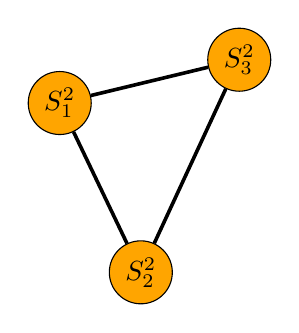
\begin{tikzpicture}[auto,vertex/.append style={minimum width=8mm}]
  \node[vertex,fill=Orange,text=black] (ms1) at (.72,-.25) {$S_1^2$};
  \node[vertex,fill=Orange,text=black] (ms2) at (1.75,-2.4) {$S_2^2$};
  \node[vertex,fill=Orange,text=black] (ms3) at (3,.3) {$S_3^2$};
  \foreach \source/\dest in {1/2, 1/3, 2/3}
  \draw[edge] (ms\source) -- (ms\dest);
\end{tikzpicture}
\end{document}
